\subsubsection{Criterios de Diseño}

\begin{itemize}
\bigskip 

\item  Caminos de los conductores de alimentación suficientemente anchos y  dispuestos uno próximo al otro, con el objetivo de disminuir el área efectiva y por lo tanto la impedancia.

\item Capacitores de desacople del valor adecuado, de modo que funcionen a la frecuencia correspondiente.

\item Líneas de señal generando la menor área compatible con la distribución de los elementos con su camino de retorno. Especialmente los caminos de alta corriente y/o velocidad como para líneas de gran sensibilidad.

\item Área efectiva del circuito lo más pequeña posible.

\item Conexiones de masas y alimentación sin bucles.

\item Capacidades parásitas entre masa y las líneas de señal minimizadas al alejar pistas.

\item Masas de entrada y salida unidas a un solo punto en común.

\item Disipadores en el borde de la placa para facilitar instalación y optimizar su disipación.

\end{itemize}

\subsubsection{Circuito Implementado}
\begin{figure}[H]
\centerline{
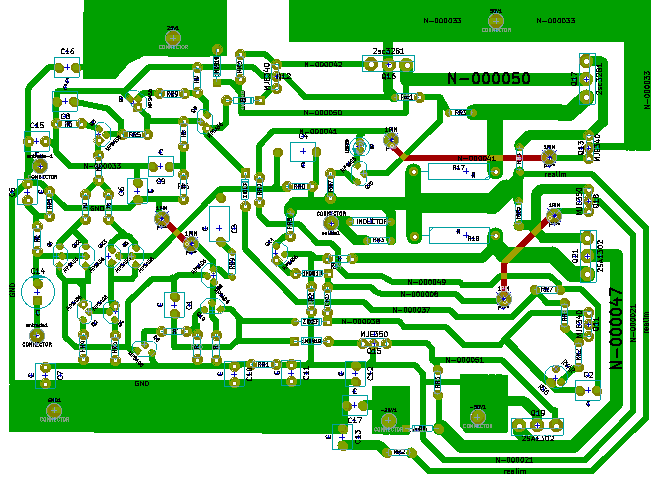
\includegraphics[scale=0.55]{img/circuito_implementado_todo.png}}
\caption{Circuito impreso del amplificador}
\end{figure}

\subsubsection{Fuente Lineal}
\medskip
Para este circuito se utilizaron pistas de 4mm de ancho. Los diodos utilizados en el puente son 6A10 los cuales pueden soportar las corrientes requeridas por el amplificador, ya que soportan hasta 6A; y poseen una caída de tension en directa menor a 1V.
En la Figura~\ref{circuito_impreso_fuente_lineal} se muestra el circuito impreso implementado. 

\begin{figure}[H]
\centering
\centerline{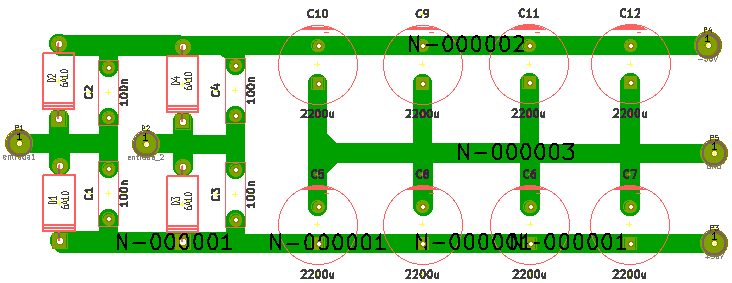
\includegraphics[scale=0.53]{img/circuito_impreso_fuente_lineal.png}}
\caption{Circuito impreso de la fuente lineal}
\label{circuito_impreso_fuente_lineal} 
\end{figure}
